%!TEX root = ../../main.tex
\chapter{性能評価・考察}
本研究の評価として,システムの操作性と推薦機構の評価実験を行った.

\section{システムの操作性の比較実験}
先行研究であるゴオルシェアと,私が開発しているミッションフォレストとの,操作性の比較実験を行った.

\subsection{実験内容}
サンプルとして\ref{img:experiment_question}に示すプロジェクトを提示し,ゴオルシェア及びミッションフォレスト両システムで作成してもった.
実際に作成されたツリーを,\ref{img:experiment_goalshare}と\ref{img:experiment_missionforest}に示す.
ウェブユーザビリティ評価スケール(WUS)に基づく評価項目\ref{table:experiment_question}について,どちらのシステムがよかったか評価してもらった.

\begin{figure}[t]
	\begin{center}
		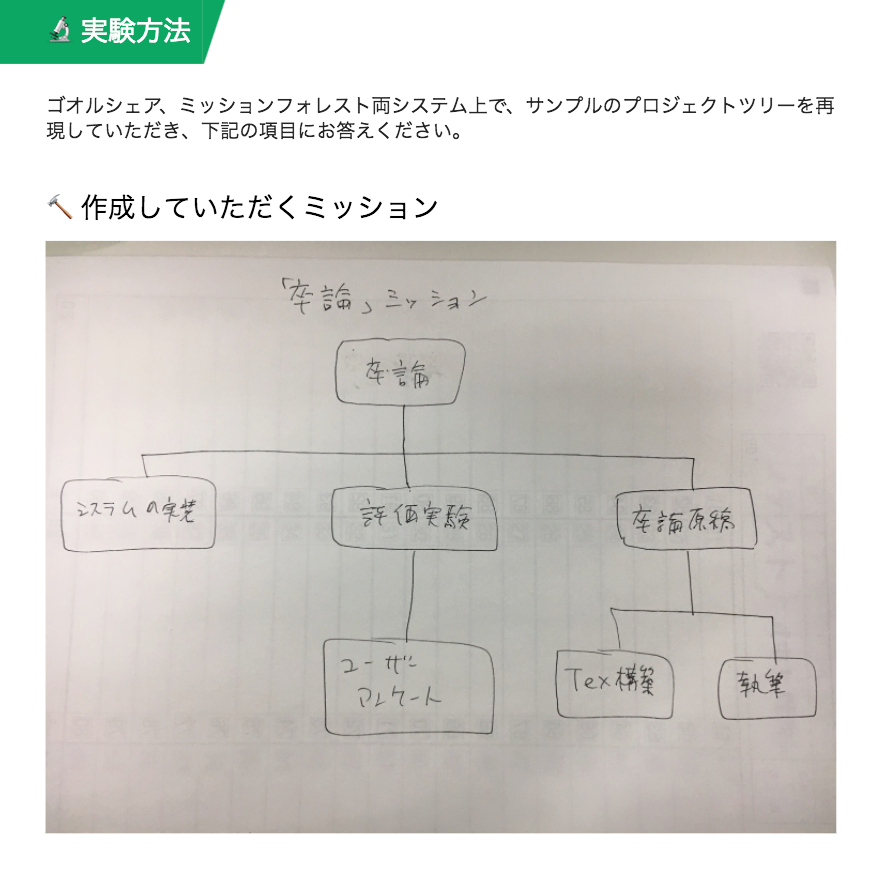
\includegraphics[width=0.9\linewidth]{assets/img/experiment_question.png}
		\caption{評価実験例題}
		\label{img:experiment_question}
	\end{center}
\end{figure}

\begin{figure}[t]
	\begin{center}
		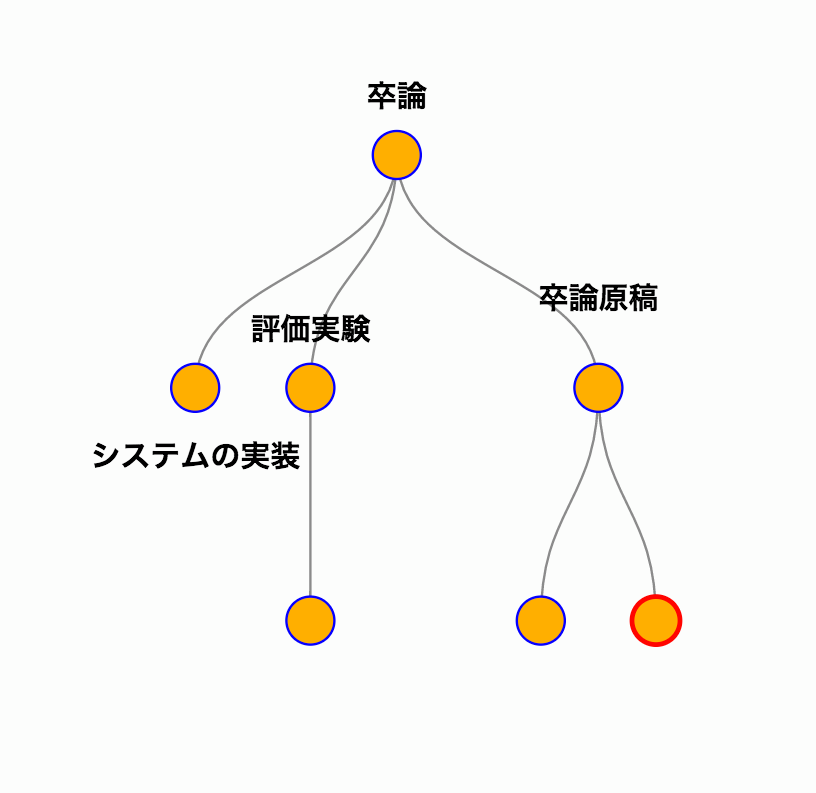
\includegraphics[width=0.9\linewidth]{assets/img/experiment_goalshare.png}
		\caption{ゴオルシェア実験結果}
		\label{img:experiment_goalshare}
	\end{center}
\end{figure}

\begin{figure}[t]
	\begin{center}
		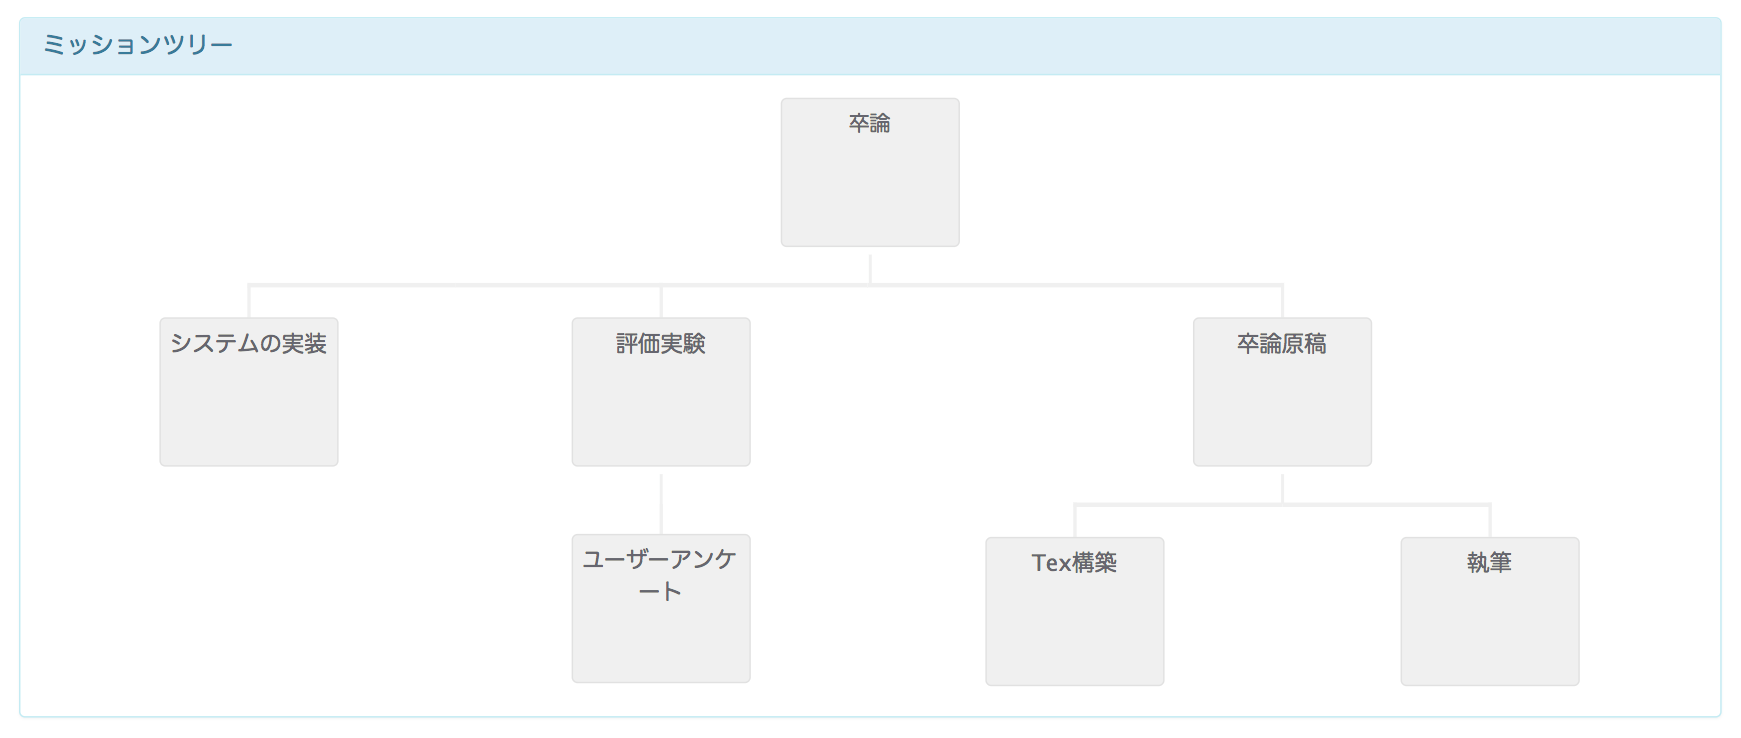
\includegraphics[width=0.9\linewidth]{assets/img/experiment_missionforest.png}
		\caption{ミッションフォレスト実験結果}
		\label{img:experiment_missionforest}
	\end{center}
\end{figure}

\begin{table}[t]
 \caption{評価実験項目}
 \begin{center}
	 \begin{tabular}{ | c | c | } \hline
			1 & ミッションの作成はどちらが操作しやすかったですか \\ \hline
 			2 & タスクの作成はどちらが操作しやすかったですか \\ \hline
 			3 & 画面上のUI構成はどちらがわかりやすかったですか \\ \hline
 			4 & どちらのツリー表示が見やすかったですか \\ \hline
 			5 & 軽快な動きをするのはどちらでしたか \\ \hline
 			6 & 今後どちらのシステムを使いたいですか \\ \hline
	 \end{tabular}
	 \label{table:experiment_question}
 \end{center}
\end{table}

\subsection{実験結果と考察}
今回はサンプルとして,10名の被験者に評価実験を行ってもらった.
以下に各評価項目ごとの結果と考察を述べる.

\subsubsection{(1)ミッションの作成はどちらが操作しやすかったですか}
TODO: エラーバーグラフ

\subsubsection{(2)タスクの作成はどちらが操作しやすかったですか}
TODO: エラーバーグラフ

\subsubsection{(3)画面上のUI構成はどちらがわかりやすかったですか}
TODO: エラーバーグラフ

\subsubsection{(4)どちらのツリー表示が見やすかったですか}
TODO: エラーバーグラフ

\subsubsection{(5)軽快な動きをするのはどちらでしたか}
TODO: エラーバーグラフ

\subsubsection{(6)今後どちらのシステムを使いたいですか}
TODO: エラーバーグラフ
